\section{Expansion of Maxwell's Curl Equations in Cartesian Coordinates}

The Maxwell's equations are:

\begin{align}
    \rot \Et(t) &= -\partial _t \Bt(t), \\
    \rot \Hht(t) &= \partial_t \Dt(t), \\
    \Div \Bt(t) &= 0, \\
    \Div \Dt(t) &= 0,
\end{align}
where $\partial_t\cdot = \partialDerivative{\cdot}{t}$.

The the constitutive relations are:
\begin{align}
    \Bt(t) &= \brackets{\mu_0\mu_r  (t)} \ast \Hht(t), \\
    \Dt(t) &= \brackets{\epsilon_0 \epsilon_r  (t)} \ast \Et(t),
\end{align}
where $\brackets{\cdot}$ represents a tensor.

\subsection{Normalizing the Electric Fields}
It will be adopted the conventional approach in FDTD and the electric field will be normalized as:
\begin{equation}
    \tilde{\Et}(t) = \sqrt{\cfrac{\epsilon_0}{\mu_0}}\Et(t) = \cfrac{1}{\eta_0}\Et(t).
\end{equation}
Also, from now on, the time depency $(t)$ will be ommited for cleaning notation reasons.

The other parameters related to the electric field must also be normalized:
\begin{equation}
    \tilde{\Dt} = \sqrt{\cfrac{1}{\epsilon_0\mu_0}} \Dt = c_0 \Dt.
\end{equation}

Therefore, the normalized Maxwell's equations become:

\begin{align}
    \rot \En &= -\partial _t \Bt, \\
    \rot \Hht &= \partial_t \Dn, \\
    \Div \Bt &= 0, \\
    \Div \Dn &= 0.
\end{align}


\subsection{Expanding Maxwell's Equations}

To expand the equations, it will be assumed that $\brackets{\mu_r}$ and $\brackets{\epsilon_r}$ has only diagonal terms \cite{rumpf_book}. 

The equation $\rot \En = - \cfrac{\brackets{\mu_r}}{c_0} \partial _t \Bt$ becomes:

\begin{align}
    \partial_z\En_y - \partial_y\En_z &= \cfrac{\mu_{xx}}{c_0} \partial_t \Hht_x, \\
    \partial_x\En_z - \partial_z\En_x &= \cfrac{\mu_{yy}}{c_0} \partial_t \Hht_y,\\
    \partial_y\En_x - \partial_x\En_y &= \cfrac{\mu_{zz}}{c_0} \partial_t \Hht_z.
\end{align}

The equation $\rot \Hht = \cfrac{1}{c_0} \partial _t \Dn$ becomes:

\begin{align}
    \partial_z\Hht_y - \partial_y\Hht_z &= \cfrac{1}{c_0} \partial_t \Dn_x, \\
    \partial_x\Hht_z - \partial_z\Hht_x &= \cfrac{1}{c_0} \partial_t \Dn_y, \\
    \partial_y\Hht_x - \partial_x\Hht_y &= \cfrac{1}{c_0} \partial_t \Dn_z.
\end{align}

Finally, the equation $ \Dn = \brackets{\epsilon_r} \En $ becomes:

\begin{align}
    \Dn_x &= \epsilon_{xx} \En_x, \label{eq:Dn_x}\\
    \Dn_y &= \epsilon_{yy} \En_y, \label{eq:Dn_y}\\
    \Dn_z &= \epsilon_{zz} \En_z. \label{eq:Dn_z}
\end{align}

\subsection{Notation for Curl Terms}

\begin{align}
    \CEx &= \partial_z\En_y - \partial_y\En_z, \\
    \CEy &= \partial_x\En_z - \partial_z\En_x, \\
    \CEz &= \partial_y\En_x - \partial_x\En_y.
\end{align}

\begin{align}
    \CHx &= \partial_z\Hht_y - \partial_y\Hht_z, \\
    \CHy &= \partial_x\Hht_z - \partial_z\Hht_x, \\
    \CHz &= \partial_y\Hht_x - \partial_x\Hht_y.
\end{align}

\subsection{Final Equations Form}

\begin{align}
    \CEx &= \cfrac{\mu_{xx}}{c_0} \partial_t \Hht_x, \\
    \CEy &= \cfrac{\mu_{yy}}{c_0} \partial_t \Hht_y,\\
    \CEz &= \cfrac{\mu_{zz}}{c_0} \partial_t \Hht_z.
\end{align}

\begin{align}
    \CHx &= \cfrac{1}{c_0} \partial_t \Dn_x, \\
    \CHy &= \cfrac{1}{c_0} \partial_t \Dn_y, \\
    \CHz &= \cfrac{1}{c_0} \partial_t \Dn_z.
\end{align}

\begin{align}
    \Dn_x &= \epsilon_{xx} \En_x, \label{eq:dnx_update} \\
    \Dn_y &= \epsilon_{yy} \En_y, \label{eq:dny_update} \\
    \Dn_z &= \epsilon_{zz} \En_z. \label{eq:dnz_update}
\end{align}


\section{Finite-Difference Approximation to Maxwell's Equations}

\subsection{Yee Grid}
A unit cell is constructed by dividing the 3 axis into discrete cells of size $(\dx, \dy, \dz)$. Inside this cell, it is necessary to put all the fields of the electromagnetic problem $(\Et_x, \Et_y, \Et_z, \Hht_x, \Hht_x, \Hht_z)$. Instead of putting all fields on the origin $(0, 0, 0)$, where is more intuitive, Yee proposed the following approach:



\tikzset{every picture/.style={line width=0.75pt}} %set default line width to 0.75pt        

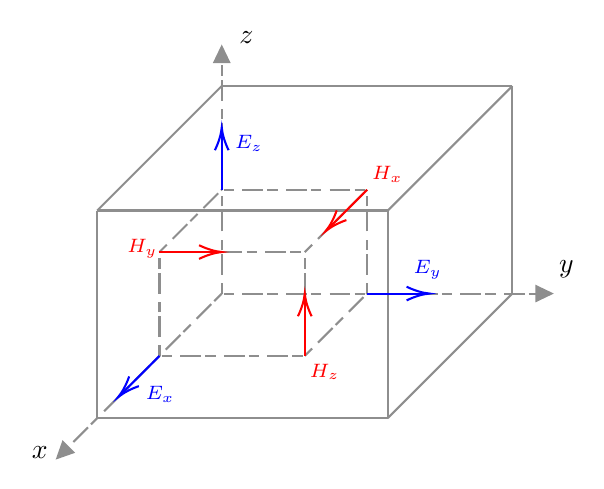
\begin{tikzpicture}[x=0.75pt,y=0.75pt,yscale=-1,xscale=1]
%uncomment if require: \path (0,300); %set diagram left start at 0, and has height of 300

%Straight Lines [id:da7206106706219195] 
\draw [color={rgb, 255:red, 142; green, 142; blue, 142 }  ,draw opacity=1 ]   (235,130) -- (235,30) ;
%Straight Lines [id:da33698179602076084] 
\draw [color={rgb, 255:red, 142; green, 142; blue, 142 }  ,draw opacity=1 ]   (35,190) -- (175,190) ;
%Straight Lines [id:da9138355462483165] 
\draw [color={rgb, 255:red, 142; green, 142; blue, 142 }  ,draw opacity=1 ]   (35,190) -- (35,90) ;
%Straight Lines [id:da685935512376388] 
\draw [color={rgb, 255:red, 142; green, 142; blue, 142 }  ,draw opacity=1 ]   (35,90) -- (175,90) ;
%Straight Lines [id:da445111134636218] 
\draw [color={rgb, 255:red, 142; green, 142; blue, 142 }  ,draw opacity=1 ]   (175,190) -- (235,130) ;
%Straight Lines [id:da484524333762936] 
\draw [color={rgb, 255:red, 142; green, 142; blue, 142 }  ,draw opacity=1 ]   (175,90) -- (235,30) ;
%Straight Lines [id:da9913295376298443] 
\draw [color={rgb, 255:red, 142; green, 142; blue, 142 }  ,draw opacity=1 ]   (35,90) -- (95,30) ;
%Straight Lines [id:da5460324336870037] 
\draw [color={rgb, 255:red, 142; green, 142; blue, 142 }  ,draw opacity=1 ]   (95,30) -- (235,30) ;
%Straight Lines [id:da6638914765185959] 
\draw [color={rgb, 255:red, 142; green, 142; blue, 142 }  ,draw opacity=1 ] [dash pattern={on 3.75pt off 3pt on 7.5pt off 1.5pt}]  (95,130) -- (95,13) ;
\draw [shift={(95,10)}, rotate = 90] [fill={rgb, 255:red, 142; green, 142; blue, 142 }  ,fill opacity=1 ][line width=0.08]  [draw opacity=0] (8.93,-4.29) -- (0,0) -- (8.93,4.29) -- cycle    ;
%Straight Lines [id:da5590643789875542] 
\draw [color={rgb, 255:red, 142; green, 142; blue, 142 }  ,draw opacity=1 ] [dash pattern={on 3.75pt off 3pt on 7.5pt off 1.5pt}]  (96,130) -- (252,130) ;
\draw [shift={(255,130)}, rotate = 180] [fill={rgb, 255:red, 142; green, 142; blue, 142 }  ,fill opacity=1 ][line width=0.08]  [draw opacity=0] (8.93,-4.29) -- (0,0) -- (8.93,4.29) -- cycle    ;
%Straight Lines [id:da13059528999125825] 
\draw [color={rgb, 255:red, 142; green, 142; blue, 142 }  ,draw opacity=1 ] [dash pattern={on 3.75pt off 3pt on 7.5pt off 1.5pt}]  (17.12,207.88) -- (95,130) ;
\draw [shift={(15,210)}, rotate = 315] [fill={rgb, 255:red, 142; green, 142; blue, 142 }  ,fill opacity=1 ][line width=0.08]  [draw opacity=0] (8.93,-4.29) -- (0,0) -- (8.93,4.29) -- cycle    ;
%Straight Lines [id:da6668538193606308] 
\draw [color={rgb, 255:red, 142; green, 142; blue, 142 }  ,draw opacity=1 ]   (175,190) -- (175,90) ;
%Straight Lines [id:da383295540871357] 
\draw [color={rgb, 255:red, 142; green, 142; blue, 142 }  ,draw opacity=1 ] [dash pattern={on 3.75pt off 3pt on 7.5pt off 1.5pt}]  (165,130) -- (165,80) ;
%Straight Lines [id:da3974993340565597] 
\draw [color={rgb, 255:red, 142; green, 142; blue, 142 }  ,draw opacity=1 ] [dash pattern={on 3.75pt off 3pt on 7.5pt off 1.5pt}]  (65,160) -- (65,110) ;
%Straight Lines [id:da44160642910672465] 
\draw [color={rgb, 255:red, 142; green, 142; blue, 142 }  ,draw opacity=1 ] [dash pattern={on 3.75pt off 3pt on 7.5pt off 1.5pt}]  (135,160) -- (135,110) ;
%Straight Lines [id:da5629234248062879] 
\draw [color={rgb, 255:red, 142; green, 142; blue, 142 }  ,draw opacity=1 ] [dash pattern={on 3.75pt off 3pt on 7.5pt off 1.5pt}]  (66,160) -- (135,160) ;
%Straight Lines [id:da5422854229817635] 
\draw [color={rgb, 255:red, 142; green, 142; blue, 142 }  ,draw opacity=1 ] [dash pattern={on 3.75pt off 3pt on 7.5pt off 1.5pt}]  (65,110) -- (135,110) ;
%Straight Lines [id:da6116059635293223] 
\draw [color={rgb, 255:red, 142; green, 142; blue, 142 }  ,draw opacity=1 ] [dash pattern={on 3.75pt off 3pt on 7.5pt off 1.5pt}]  (96,80) -- (165,80) ;
%Straight Lines [id:da9246979014557115] 
\draw [color={rgb, 255:red, 142; green, 142; blue, 142 }  ,draw opacity=1 ] [dash pattern={on 3.75pt off 3pt on 7.5pt off 1.5pt}]  (65,110) -- (95,80) ;
%Straight Lines [id:da7936751206446481] 
\draw [color={rgb, 255:red, 142; green, 142; blue, 142 }  ,draw opacity=1 ] [dash pattern={on 3.75pt off 3pt on 7.5pt off 1.5pt}]  (135,110) -- (165,80) ;
%Straight Lines [id:da5136819716767439] 
\draw [color={rgb, 255:red, 142; green, 142; blue, 142 }  ,draw opacity=1 ] [dash pattern={on 3.75pt off 3pt on 7.5pt off 1.5pt}]  (135,160) -- (165,130) ;
%Straight Lines [id:da7961144391033157] 
\draw [color={rgb, 255:red, 255; green, 0; blue, 0 }  ,draw opacity=1 ]   (65,110) -- (93,110) ;
\draw [shift={(95,110)}, rotate = 180] [color={rgb, 255:red, 255; green, 0; blue, 0 }  ,draw opacity=1 ][line width=0.75]    (10.93,-3.29) .. controls (6.95,-1.4) and (3.31,-0.3) .. (0,0) .. controls (3.31,0.3) and (6.95,1.4) .. (10.93,3.29)   ;
%Straight Lines [id:da12124972293983005] 
\draw [color={rgb, 255:red, 255; green, 0; blue, 0 }  ,draw opacity=1 ]   (165,80) -- (146.41,98.59) ;
\draw [shift={(145,100)}, rotate = 315] [color={rgb, 255:red, 255; green, 0; blue, 0 }  ,draw opacity=1 ][line width=0.75]    (10.93,-3.29) .. controls (6.95,-1.4) and (3.31,-0.3) .. (0,0) .. controls (3.31,0.3) and (6.95,1.4) .. (10.93,3.29)   ;
%Straight Lines [id:da3302622370080578] 
\draw [color={rgb, 255:red, 255; green, 0; blue, 0 }  ,draw opacity=1 ]   (135,160) -- (135,132) ;
\draw [shift={(135,130)}, rotate = 90] [color={rgb, 255:red, 255; green, 0; blue, 0 }  ,draw opacity=1 ][line width=0.75]    (10.93,-3.29) .. controls (6.95,-1.4) and (3.31,-0.3) .. (0,0) .. controls (3.31,0.3) and (6.95,1.4) .. (10.93,3.29)   ;
%Straight Lines [id:da5288808191623237] 
\draw [color={rgb, 255:red, 0; green, 0; blue, 255 }  ,draw opacity=1 ]   (95,80) -- (95,52) ;
\draw [shift={(95,50)}, rotate = 90] [color={rgb, 255:red, 0; green, 0; blue, 255 }  ,draw opacity=1 ][line width=0.75]    (10.93,-3.29) .. controls (6.95,-1.4) and (3.31,-0.3) .. (0,0) .. controls (3.31,0.3) and (6.95,1.4) .. (10.93,3.29)   ;
%Straight Lines [id:da13848590216057788] 
\draw [color={rgb, 255:red, 0; green, 0; blue, 255 }  ,draw opacity=1 ]   (65,160) -- (46.41,178.59) ;
\draw [shift={(45,180)}, rotate = 315] [color={rgb, 255:red, 0; green, 0; blue, 255 }  ,draw opacity=1 ][line width=0.75]    (10.93,-3.29) .. controls (6.95,-1.4) and (3.31,-0.3) .. (0,0) .. controls (3.31,0.3) and (6.95,1.4) .. (10.93,3.29)   ;
%Straight Lines [id:da9041413940467059] 
\draw [color={rgb, 255:red, 0; green, 0; blue, 255 }  ,draw opacity=1 ]   (165,130) -- (193,130) ;
\draw [shift={(195,130)}, rotate = 180] [color={rgb, 255:red, 0; green, 0; blue, 255 }  ,draw opacity=1 ][line width=0.75]    (10.93,-3.29) .. controls (6.95,-1.4) and (3.31,-0.3) .. (0,0) .. controls (3.31,0.3) and (6.95,1.4) .. (10.93,3.29)   ;

% Text Node
\draw (2,202.4) node [anchor=north west][inner sep=0.75pt]    {$x$};
% Text Node
\draw (256,112.4) node [anchor=north west][inner sep=0.75pt]    {$y$};
% Text Node
\draw (102,2.4) node [anchor=north west][inner sep=0.75pt]    {$z$};
% Text Node
\draw (48,102.4) node [anchor=north west][inner sep=0.75pt]  [font=\scriptsize,color={rgb, 255:red, 255; green, 0; blue, 0 }  ,opacity=1 ]  {$H_{y}$};
% Text Node
\draw (136,162.4) node [anchor=north west][inner sep=0.75pt]  [font=\scriptsize,color={rgb, 255:red, 255; green, 0; blue, 0 }  ,opacity=1 ]  {$H_{z}$};
% Text Node
\draw (166,67.4) node [anchor=north west][inner sep=0.75pt]  [font=\scriptsize,color={rgb, 255:red, 255; green, 0; blue, 0 }  ,opacity=1 ]  {$H_{x}$};
% Text Node
\draw (57,173.4) node [anchor=north west][inner sep=0.75pt]  [font=\scriptsize,color={rgb, 255:red, 0; green, 0; blue, 255 }  ,opacity=1 ]  {$E_{x}$};
% Text Node
\draw (186,112.4) node [anchor=north west][inner sep=0.75pt]  [font=\scriptsize,color={rgb, 255:red, 0; green, 0; blue, 255 }  ,opacity=1 ]  {$E_{y}$};
% Text Node
\draw (100,52.4) node [anchor=north west][inner sep=0.75pt]  [font=\scriptsize,color={rgb, 255:red, 0; green, 0; blue, 255 }  ,opacity=1 ]  {$E_{z}$};


\end{tikzpicture}


\begin{itemize}
    \item $\Et_x$ on $(\dx/2, 0, 0)$,
    \item $\Et_y$ on $(0, \dy/2, 0)$,
    \item $\Et_z$ on $(0, 0, \dz/2)$,
    \item $\Hht_x$ on $(0, \dy/2, \dz/2)$,
    \item $\Hht_y$ on $(\dx/2, 0, \dz/2)$,
    \item $\Hht_z$ on $(\dx/2, \dy/2, 0)$.
\end{itemize}

There are some reasons for using this scheme:
\begin{itemize}
    \item The divergences are naturally zero.
    \item The physical boundary conditions are naturally satisfied.
    \item It is an elegant arrangement to approximate Maxwell's curl equations.
\end{itemize}

Additionaly, there are some consequences for using this scheme:
\begin{itemize}
    \item Field components are in physically different locations.
    \item Field components may be in different materials even if they are in the same unit cell.
    \item Field components will be out of phase.
\end{itemize}

\subsection{Finite-Difference Equations on Yee Grid}

Each cell on the grid is identified by the coordines $(i\dx, j\dy, k\dz)$, where $(i, j, k)$ are the index of the cell.

Note that on each face of the Yee cell there is the fields of the adjacent cell.

Consider, first, the grid for $\Hht_x$:

\input{contents/tiks/yee_grid_chx.tex}

Based on this schematic, it is possible to write \cite{rumpf_book}:

\begin{align}
    \partialDerivative{\En_z\Big|^{i,j,k}_t}{y} =& \cfrac{\En_z\Big|^{i,j+1,k}_t-\En_z\Big|^{i,j,k}_t}{\dy}, \\
    \partialDerivative{\En_y\Big|^{i,j,k}_t}{z} =& \cfrac{\En_y\Big|^{i,j,k+1}_t-\En_y\Big|^{i,j,k}_t}{\dy}.
\end{align}

Note that this space derivatives exists at time instant $t$ and they exist at the same point as $\Hht_x^{i,j,k}$.

We need to explicitly write the time on the Yee grid equations, since it is essencial to write all the members of equations on the same time instant.

Hence, the $\CEx$ final equation is:

\begin{align}
    \resizebox{.8\hsize}{!}{$
        \CEx = \cfrac{\En_z\Big|^{i,j+1,k}_t-\En_z\Big|^{i,j,k}_t}{\dy} - \cfrac{\En_y\Big|^{i,j,k+1}_t-\En_y\Big|^{i,j,k}_t}{\dz}
        \label{eq:CEx}
    $}
\end{align}


Now, for the time derivative $\partial_t \Hht_x$ to exists at time $t$:

\begin{equation}
    \partial_t \Hht_x\Big|^{i,j,k}_t = \cfrac{\Hht_x\Big|^{i,j,k}_{t+\nicefrac{\dt}{2}} - \Hht_x\Big|^{i,j,k}_{t-\nicefrac{\dt}{2}}}{\dt}.
\end{equation}

So, the finite-difference equation for $\Hht_x$ becomes:

\begin{align}
    \cfrac{\En_z\Big|^{i,j+1,k}_{t}-\En_z\Big|^{i,j,k}_{t}}{\dy} - \cfrac{\En_y\Big|^{i,j,k+1}_{t}-\En_y\Big|^{i,j,k}_{t}}{\dy} \nonumber \\ 
    =\cfrac{\mu_{xx}\Big|^{i,j,k}}{c_0}\cfrac{\Hht_x\Big|^{i,j,k}_{t+\nicefrac{\dt}{2}} - \Hht_x\Big|^{i,j,k}_{t-\nicefrac{\dt}{2}}}{\dt}.
    \label{eq:fd_hx}
\end{align}

Similarly, it is possible to write the curl equations for the other components of $\En$ and for $\Hht$:



\begin{align}
    \resizebox{.8\hsize}{!}{$
    \CEy = \cfrac{\En_x\Big|^{i,j,k+1}_{t}-\En_x\Big|^{i,j,k}_{t}}{\dz} - \cfrac{\En_z\Big|^{i+1,j,k}_{t}-\En_z\Big|^{i,j,k}_{t}}{\dx}
    \label{eq:CEy}
    $}
\end{align}

\begin{align}
    \resizebox{.8\hsize}{!}{$
        \CEz = \cfrac{\En_y\Big|^{i+1,j,k}_{t}-\En_y\Big|^{i,j,k}_{t}}{\dx} - \cfrac{\En_x\Big|^{i,j+1,k}_{t}-\En_x\Big|^{i,j,k}_{t}}{\dy}
        \label{eq:CEz}
    $}
\end{align}

\begin{align}
    \resizebox{.8\hsize}{!}{$
        \CHx = \cfrac{\Hht_z\Big|^{i,j,k}_{t+\nicefrac{\dt}{2}}-\Hht_z\Big|^{i,j-1,k}_{t+\nicefrac{\dt}{2}}}{\dy} - \cfrac{\Hht_y\Big|^{i,j,k}_{t+\nicefrac{\dt}{2}}-\Hht_y\Big|^{i,j,k-1}_{t+\nicefrac{\dt}{2}}}{\dz}
        \label{eq:CHx}
    $}
\end{align}


\begin{align}
    \resizebox{.8\hsize}{!}{$
        \CHy = \cfrac{\Hht_x\Big|^{i,j,k}_{t+\nicefrac{\dt}{2}}-\Hht_x\Big|^{i,j,k-1}_{t+\nicefrac{\dt}{2}}}{\dz} - \cfrac{\Hht_z\Big|^{i,j,k}_{t+\nicefrac{\dt}{2}}-\Hht_z\Big|^{i-1,j,k}_{t+\nicefrac{\dt}{2}}}{\dx}
        \label{eq:CHy}
    $}
\end{align}


\begin{align}
    \resizebox{.8\hsize}{!}{$
        \CHz = \cfrac{\Hht_y\Big|^{i,j,k}_{t+\nicefrac{\dt}{2}}-\Hht_y\Big|^{i-1,j,k}_{t+\nicefrac{\dt}{2}}}{\dx} - \cfrac{\Hht_x\Big|^{i,j,k}_{t+\nicefrac{\dt}{2}}-\Hht_x\Big|^{i,j-1,k}_{t+\nicefrac{\dt}{2}}}{\dy}
        \label{eq:CHz}
    $}
\end{align}


Finally, the finite-difference equations are, for $\Hht_y$:

\begin{align}
    \cfrac{\En_x\Big|^{i,j,k+1}_{t}-\En_x\Big|^{i,j,k}_{t}}{\dz} - \cfrac{\En_z\Big|^{i+1,j,k}_{t}-\En_z\Big|^{i,j,k}_{t}}{\dx} \nonumber \\ 
    =\cfrac{\mu_{yy}\Big|^{i,j,k}}{c_0}\cfrac{\Hht_y\Big|^{i,j,k}_{t+\dttwo} - \Hht_y\Big|^{i,j,k}_{t-\dttwo}}{\dt},
    \label{eq:fd_hy}
\end{align}

for $\Hht_z$:

\begin{align}
    \cfrac{\En_y\Big|^{i+1,j,k}_{t}-\En_y\Big|^{i,j,k}_{t}}{\dx} - \cfrac{\En_x\Big|^{i,j+1,k}_{t}-\En_x\Big|^{i,j,k}_{t}}{\dy} \nonumber \\
    =\cfrac{\mu_{zz}^{i,j,k}}{c_0}\cfrac{\Hht_z\Big|^{i,j,k}_{t+\dttwo} - \Hht_z\Big|^{i,j,k}_{t-\dttwo}}{\dt},
    \label{eq:fd_hz}
\end{align}

for $\En_x$:

\begin{small}
    \begin{align}
        \cfrac{\Hht_z\Big|^{i,j,k}_{t+\dttwo}-\Hht_z\Big|^{i,j-1,k}_{t+\dttwo}}{\dy} - \cfrac{\Hht_y\Big|^{i,j,k}_{t+\dttwo}-\Hht_y\Big|^{i,j,k-1}_{t+\dttwo}}{\dz} \nonumber\\
        =
        \cfrac{\epsilon_{xx}\Big|^{i,j,k}}{c_0}\cfrac{\En_x\Big|^{i,j,k}_{t+\dt}-\En_x\Big|^{i,j,k}_{t}}{\dt},
        \label{eq:fd_ex}
    \end{align}  
\end{small}


for $\En_y$:

\begin{small}
    \begin{align}
        \cfrac{\Hht_x\Big|^{i,j,k}_{t+\dttwo}-\Hht_x\Big|^{i,j,k-1}_{t+\dttwo}}{\dz} - \cfrac{\Hht_z\Big|^{i,j,k}_{t+\dttwo}-\Hht_z\Big|^{i-1,j,k}_{t+\dttwo}}{\dx} \nonumber\\ =
        \cfrac{\epsilon_{yy}\Big|^{i,j,k}}{c_0}\cfrac{\En_y\Big|^{i,j,k}_{t+\dt}-\En_y\Big|^{i,j,k}_{t}}{\dt},
        \label{eq:fd_ey}
    \end{align}
\end{small}
and for $\En_z$:

\begin{small}
    \begin{align}
        \cfrac{\Hht_y\Big|^{i,j,k}_{t+\dttwo}-\Hht_y\Big|^{i-1,j,k}_{t+\dttwo}}{\dx} - \cfrac{\Hht_x\Big|^{i,j,k}_{t+\dttwo}-\Hht_x\Big|^{i,j-1,k}_{t+\dttwo}}{\dy} \nonumber\\
        =
        \cfrac{\epsilon_{zz}\Big|^{i,j,k}}{c_0}\cfrac{\En_z\Big|^{i,j,k}_{t+\dt}-\En_z\Big|^{i,j,k}_{t}}{\dt}.
        \label{eq:fd_ez}
    \end{align}
\end{small}

To ease the implementation, the vector $\En$ will exists at integer step times $(0, \dt, 2\dt, \dots)$ meanwhile the vector $\Hht$ will exists at half time steps $(\nicefrac{\dt}{2}, 3\nicefrac{\dt}{2}, 5\nicefrac{\dt}{2}, \dots)$.

\section{The Perfect Matching Layer}

The tensors for the permittivity and permeability will be \cite{rumpf_book}:

\begin{equation}
    \brackets{\epsilon_{r,x}} = \brackets{\mu_{r,x}} = \begin{bmatrix}
        \cfrac{1}{s_x} & 0 & 0 \\
        0 & s_x & 0 \\
        0 & 0 & s_x
    \end{bmatrix},
\end{equation}
for a wave travelling at $x$ direction,

\begin{equation}
    \brackets{\epsilon_{r,y}} = \brackets{\mu_{r,y}} = \begin{bmatrix}
        s_y & 0 & 0 \\
        0 & \cfrac{1}{s_y} & 0 \\
        0 & 0 & s_y
    \end{bmatrix},
\end{equation}
for a wave travelling at $y$ direction, and

\begin{equation}
    \brackets{\epsilon_{r,z}} = \brackets{\mu_{r,z}} = \begin{bmatrix}
        s_z & 0 & 0 \\
        0 & s_z & 0 \\
        0 & 0 & \cfrac{1}{s_z}
    \end{bmatrix},
\end{equation}
for a wave travelling at $z$ direction.

The loss is incorporated into the permittivity through the electrical conductivity $\sigma$ as $\tilde{\epsilon} = \epsilon_r + \cfrac{\sigma}{j\omega \epsilon_0}$. 

And, for absorbing all waves in all boundaries, that is achieved by matching the impedance and incorporating loss in all directions:

\begin{equation}
    \brackets{\epsilon_{r,\textnormal{UPML}}} = \brackets{\mu_{r,\textnormal{UPML}}} = \brackets{S} = \brackets{\epsilon_{r,x}}\brackets{\epsilon_{r,y}}\brackets{\epsilon_{r,z}} \nonumber
\end{equation} 
\begin{equation}
    \brackets{S} = \begin{bmatrix}
        \cfrac{s_ys_z}{s_x} & 0 & 0 \\
        0 & \cfrac{s_xs_z}{s_y} & 0 \\
        0 & 0 & \cfrac{s_xs_y}{s_z}
    \end{bmatrix}.
\end{equation}



\subsection{The PML Parameters}

Considering $\epsilon_r = 1$, the parameters $s_i$ are \cite{rumpf_book}:

\begin{align}
    s_i = 1 + \cfrac{\sigma_i\Prime}{j\omega\epsilon_0}, i \in (x, y, z)
\end{align}

And the fake conductivities are:

\begin{align}
    \sigma_x\Prime(x) &= \cfrac{\epsilon_0}{2\dt}\pare{\cfrac{x}{L_x}}^3 \\
    \sigma_y\Prime(y) &= \cfrac{\epsilon_0}{2\dt}\pare{\cfrac{y}{L_y}}^3 \\
    \sigma_z\Prime(z) &= \cfrac{\epsilon_0}{2\dt}\pare{\cfrac{z}{L_z}}^3
\end{align}
where $L_i$ is the length of the PML extending in the $i$ direction.


\subsection{Incorporating PML into Maxwell's Equations}

The Maxwell's Equations in the frequency domain are:

\begin{align}
    \rot \E (\omega) &= -j\omega \mu_0 \brackets{\mu_r} \Hh (\omega) \\
    \rot \Hh (\omega) &= \sigma \E(\omega) + j\omega\brackets{S} \D (\omega) \\
    \D (\omega) &= \epsilon_0 \brackets{\epsilon _r}\E (\omega)
\end{align}

The PML $\brackets{S}$ can be incorporated as:

\begin{align}
    \rot \E (\omega) &= -j\omega \mu_0 \brackets{\mu_r} \brackets{S} \Hh (\omega) \\
    \rot \Hh (\omega) &= \sigma \E(\omega) + j\omega \D (\omega) \\
    \D (\omega) &= \epsilon_0 \brackets{\epsilon _r} \E (\omega)
\end{align}

Normalizing the electric field:

\begin{equation}
    \tilde{\E}(\omega) = \sqrt{\cfrac{\epsilon_0}{\mu_0}}\E(\omega) = \cfrac{1}{\eta_0}\E(\omega)
\end{equation}

\begin{equation}
    \tilde{\D}(\omega) = \sqrt{\cfrac{1}{\epsilon_0\mu_0}} \D(\omega) = c_0 \D(\omega)
\end{equation}

Hence, the equations become:

\begin{align}
    \rot \Enw (\omega) &= -j\omega\cfrac{\brackets{\mu_r}}{c_0} \brackets{S} \Hh (\omega) \\
    \rot \Hh (\omega) &= \eta_0 \sigma \Enw(\omega) + \cfrac{j\omega}{c_0}\brackets{S} \Dnw (\omega) \\
    \D (\omega) &= \brackets{\epsilon _r} \Enw (\omega)
\end{align}

Keeping $\brackets{S}$ separate from $\brackets{\mu_r}$ and $\brackets{\epsilon_r}$ allows the PML to be handled independently from the materials being simulated.

The $\omega$ will be ommitted from the equations.

Considering only the diagonal terms in $\brackets{\mu_r}$, $\brackets{\epsilon_r}$ and $\brackets{\sigma}$ = 0, the final form of the Maxwell's Equations with UPML are \cite{empossible_3d_pml}:

\begin{small}

    \begin{align}
        &j\omega\pare{1 + \cfrac{\sigma_x\Prime}{j\omega\epsilon_0}}\inverse \pare{1 + \cfrac{\sigma_y\Prime}{j\omega\epsilon_0}}\pare{1 + \cfrac{\sigma_z\Prime}{j\omega\epsilon_0}} \Hh_x \nonumber \\
        &= -\cfrac{c_0}{\mu_{xx}}\CExw
        \label{eq:Hx_upml_freq}
    \end{align}

    \begin{align}
        &j\omega\pare{1 + \cfrac{\sigma_x\Prime}{j\omega\epsilon_0}} \pare{1 + \cfrac{\sigma_y\Prime}{j\omega\epsilon_0}}\inverse\pare{1 + \cfrac{\sigma_z\Prime}{j\omega\epsilon_0}} \Hh_y \nonumber \\
        &= -\cfrac{c_0}{\mu_{yy}}\CEyw
        \label{eq:Hy_upml_freq}
    \end{align}

    \begin{align}
        &j\omega\pare{1 + \cfrac{\sigma_x\Prime}{j\omega\epsilon_0}} \pare{1 + \cfrac{\sigma_y\Prime}{j\omega\epsilon_0}}\pare{1 + \cfrac{\sigma_z\Prime}{j\omega\epsilon_0}}\inverse \Hh_z \nonumber \\
        &= -\cfrac{c_0}{\mu_{zz}}\CEzw
        \label{eq:Hz_upml_freq}
    \end{align}

    \begin{align}
        &j\omega\pare{1 + \cfrac{\sigma_x\Prime}{j\omega\epsilon_0}}\inverse \pare{1 + \cfrac{\sigma_y\Prime}{j\omega\epsilon_0}}\pare{1 + \cfrac{\sigma_z\Prime}{j\omega\epsilon_0}} \Dnw_x \nonumber \\
        &= c_0\CHxw - \cfrac{\sigma_{xx}}{\epsilon_0}\Enw_x
        \label{eq:Ex_upml_freq}
    \end{align}

    \begin{align}
        &j\omega\pare{1 + \cfrac{\sigma_x\Prime}{j\omega\epsilon_0}} \pare{1 + \cfrac{\sigma_y\Prime}{j\omega\epsilon_0}}\inverse \pare{1 + \cfrac{\sigma_z\Prime}{j\omega\epsilon_0}} \Dnw_y \nonumber \\
        &= c_0\CHyw - \cfrac{\sigma_{yy}}{\epsilon_0}\Enw_y
        \label{eq:Ey_upml_freq}
    \end{align}

    \begin{align}
        &j\omega\pare{1 + \cfrac{\sigma_x\Prime}{j\omega\epsilon_0}} \pare{1 + \cfrac{\sigma_y\Prime}{j\omega\epsilon_0}} \pare{1 + \cfrac{\sigma_z\Prime}{j\omega\epsilon_0}}\inverse \Dnw_z \nonumber \\
        &= c_0\CHzw - \cfrac{\sigma_{zz}}{\epsilon_0}\Enw_z
        \label{eq:Ez_upml_freq}
    \end{align}

    \begin{align}
        \Dnw_x =& \epsilon_{xx} \Enw_x, \\
        \Dnw_y =& \epsilon_{yy} \Enw_y, \\
        \Dnw_z =& \epsilon_{zz} \Enw_z. 
    \end{align}

\end{small}

\subsection{Conversion to the Time-Domain}
% First, assume no conductivity: $\brackets{\sigma} = 0$.

Starting from \eqref{eq:Hx_upml_freq}:


\begin{align}
    j\omega \Hh_x + \cfrac{\sigma_y\Prime + \sigma_z\Prime}{\epsilon_0}\Hh_x + \cfrac{1}{j\omega}\cfrac{\sigma_y\Prime\sigma_z\Prime}{\epsilon_0^2}\Hh_x \nonumber \\
    = -\cfrac{c_0}{\mu_{xx}}\CExw - \cfrac{1}{j\omega}\cfrac{c_0\sigma_x\Prime}{\epsilon_0\mu_{xx}}\CExw
\end{align}

In the time-domain becomes:

\begin{align}
    \partial_t\Hht_x + \cfrac{\sigma_y\Prime + \sigma_z\Prime}{\epsilon_0}\Hht_x + \int\limits_{-\infty}^t\cfrac{\sigma_y\Prime\sigma_z\Prime}{\epsilon_0^2}\Hht_x(\tau)d\tau \nonumber \\
    = -\cfrac{c_0}{\mu_{xx}}\CEx - \int\limits_{\infty}^t\cfrac{c_0\sigma_x\Prime}{\epsilon_0\mu_{xx}}\CEx(\tau)d\tau
    \label{eq:Hx_upml_time}
\end{align}

Similarly, for the other components:

\begin{align}
    \partial_t\Hht_y &+ \cfrac{\sigma_x\Prime + \sigma_z\Prime}{\epsilon_0}\Hht_y + \int\limits_{-\infty}^t\cfrac{\sigma_x\Prime\sigma_z\Prime}{\epsilon_0^2}\Hht_y(\tau)d\tau \nonumber \\
    &= -\cfrac{c_0}{\mu_{yy}}\CEy - \int\limits_{\infty}^t\cfrac{c_0\sigma_y\Prime}{\epsilon_0\mu_{yy}}\CEy(\tau)d\tau
    \label{eq:Hy_upml_time}
\end{align}

\begin{align}
    \partial_t\Hht_z
    &+
    \cfrac{\sigma_x\Prime + \sigma_y\Prime}{\epsilon_0}\Hht_z
    +
    \int\limits_{-\infty}^t\cfrac{\sigma_x\Prime\sigma_y\Prime}{\epsilon_0^2}\Hht_z(\tau)d\tau \nonumber \\
    &= 
    -\cfrac{c_0}{\mu_{zz}}\CEz
    -\int\limits_{\infty}^t\cfrac{c_0\sigma_z\Prime}{\epsilon_0\mu_{zz}}\CEz(\tau)d\tau
    \label{eq:Hz_upml_time}
\end{align}

\begin{align}
    \partial_t\Dn_x
    &+
    \cfrac{\sigma_y\Prime + \sigma_z\Prime}{\epsilon_0}\Dn_x
    +
    \cfrac{\sigma_y\Prime \sigma_z\Prime}{\epsilon_0^2} \int\limits_{-\infty}^t\Dn_x(\tau)d\tau 
    \nonumber \\
    &=
    c_0\CHx
    +
    \cfrac{c_0\sigma_x\Prime}{\epsilon_0}\int\limits_{-\infty}^t\CHx(\tau)d\tau
    \label{eq:Dx_upml_time}
\end{align}

\begin{align}
    \partial_t\Dn_y
    &+
    \cfrac{\sigma_x\Prime + \sigma_z\Prime}{\epsilon_0}\Dn_y
    +
    \cfrac{\sigma_x\Prime \sigma_z\Prime}{\epsilon_0^2} \int\limits_{-\infty}^t\Dn_y(\tau)d\tau 
    \nonumber \\
    &=
    c_0\CHy
    +
    \cfrac{c_0\sigma_y\Prime}{\epsilon_0}\int\limits_{-\infty}^t\CHy(\tau)d\tau
    \label{eq:Dy_upml_time}
\end{align}

\begin{align}
    \partial_t\Dn_z
    &+
    \cfrac{\sigma_x\Prime + \sigma_y\Prime}{\epsilon_0}\Dn_z
    +
    \cfrac{\sigma_x\Prime \sigma_y\Prime}{\epsilon_0^2} \int\limits_{-\infty}^t\Dn_z(\tau)d\tau 
    \nonumber \\
    &=
    c_0\CHz
    +
    \cfrac{c_0\sigma_z\Prime}{\epsilon_0}\int\limits_{-\infty}^t\CHz(\tau)d\tau
    \label{eq:Dz_upml_time}
\end{align}

The update equations for $\Dn$ are the same as \eqref{eq:dnx_update}, \eqref{eq:dny_update} and \eqref{eq:dnz_update}.

\subsection{Numerical Approximations}

Remark: Yee cell will be considered for numerical implementation.

Starting from \eqref{eq:Hx_upml_time}, each term of equation will be approximated as shown.

For the term 1, the time approximation will be the same as used before:

\begin{align}
    \partial_t\Hht_x(t) \approx \cfrac{\Hht_x\Big|_{(t+\nicefrac{\dt}{2})}^{i,j,k}-\Hht_x\Big|^{i,j,k}_{(t-\nicefrac{\dt}{2})}}{\dt}
\end{align}

For the term 2, it is necessary to approximate $\Hht_x(t)$, that will be done by averaging the values at $t + \nicefrac{\dt}{2}$ and $t - \nicefrac{\dt}{2}$:

\begin{align}
    \resizebox{.9\hsize}{!}{$
    \cfrac{\sigma_y\Prime + \sigma_z\Prime}{\epsilon_0}\Hht_x(t)\approx
    \cfrac{\sigma_y\Prime + \sigma_z\Prime}{\epsilon_0}\cfrac{\Hht_x\Big|_{(t+\nicefrac{\dt}{2})}^{i,j,k}+\Hht_x\Big|^{i,j,k}_{(t-\nicefrac{\dt}{2})}}{2}
    $}
\end{align}

For the term 3, it is necessary to approximate the integral with a summation:

\begin{align}
    \int\limits_{-\infty}^t\cfrac{\sigma_y\Prime\sigma_z\Prime}{\epsilon_0^2}\Hht_x(\tau)d\tau \approx \cfrac{\sigma_y\Prime\sigma_z\Prime}{\epsilon_0^2} \sum_{T=\nicefrac{\dt}{2}}^{t + \nicefrac{\dt}{2}}\Hht_x\Big|^{i,j,k}_{T}\dt
\end{align}

However, in this way the summation is going future on time. The fix is simple: just pull out the last term from summation and do the integration over half a time step:

\begin{align}
    &\int\limits_{-\infty}^t\cfrac{\sigma_y\Prime\sigma_z\Prime}{\epsilon_0^2}\Hht_x(\tau)d\tau \nonumber \\ \nonumber
    &\approx \cfrac{\sigma_y\Prime\sigma_z\Prime}{\epsilon_0^2} \left( \Hht_x\Big|_{(t+\nicefrac{\dt}{2})}^{i,j,k} \cfrac{\dt}{2} + \sum\limits_{T=\nicefrac{\dt}{2}}^{t - \nicefrac{\dt}{2}}\Hht_x\Big|^{i,j,k}_{T}\dt \right) \\ \nonumber
    &\approx\cfrac{\sigma_y\Prime\sigma_z\Prime\dt}{\epsilon_0^2} \left( \cfrac{\Hht_x\Big|_{(t+\nicefrac{\dt}{2})}^{i,j,k}-\Hht_x\Big|^{i,j,k}_{(t-\nicefrac{\dt}{2})}}{4} \right. \\ & \left. + \sum\limits_{T=\nicefrac{\dt}{2}}^{t - \nicefrac{\dt}{2}}\Hht_x\Big|^{i,j,k}_{T} \right)
\end{align}


For the term 4, the curl approximation for will be the same as in \eqref{eq:CEx}:

\begin{align}
    -\cfrac{c_0}{\mu_{xx}}\CEx \approx -\cfrac{c_0}{\mu_{xx}\Big|^{i,j,k}}\CEx\Big|^{i,j,k}_{t}
\end{align}

For the term 5, as for the term 3, the integral will be approximated with a summation:

\begin{align}
    - \int\limits_{\infty}^t\cfrac{c_0\sigma_x\Prime}{\epsilon_0\mu_{xx}}\CEx(\tau)d\tau = - \cfrac{c_0\sigma_x\Prime}{\epsilon_0\mu_{xx}} \int\limits_{\infty}^t\CEx(\tau)d\tau \nonumber \\
    \approx - \cfrac{c_0\sigma_x^H\Big|^{i,j,k}}{\epsilon_0\mu_{xx}\Big|^{i,j,k}} \sum\limits_{T=0}^{t}\CEx\Big|^{i,j,k}_{T}\dt \nonumber \\
    \approx - \cfrac{c_0\dt\sigma_x^H\Big|^{i,j,k}}{\epsilon_0\mu_{xx}\Big|^{i,j,k}} \sum\limits_{T=0}^{t}\CEx\Big|^{i,j,k}_{T}
\end{align}

\subsection{Update equations}

Starting from the numerical approximation of \eqref{eq:Hx_upml_time}:

\begin{small}
    \begin{align}
        &\cfrac{\Hht_x\Big|_{(t+\nicefrac{\dt}{2})}^{i,j,k}-\Hht_x\Big|^{i,j,k}_{(t-\nicefrac{\dt}{2})}}{\dt} \nonumber \\ 
        &+ \cfrac{\sigma_y\Prime + \sigma_z\Prime}{\epsilon_0}\cfrac{\Hht_x\Big|_{(t+\nicefrac{\dt}{2})}^{i,j,k}+\Hht_x\Big|^{i,j,k}_{(t-\nicefrac{\dt}{2})}}{2}  \nonumber \\
        &= -\cfrac{c_0}{\mu_{xx}\Big|^{i,j,k}}\CEx\Big|^{i,j,k}_{t} - \cfrac{c_0\dt\sigma_x^H\Big|^{i,j,k}}{\epsilon_0\mu_{xx}\Big|^{i,j,k}} \sum\limits_{T=0}^{t}\CEx\Big|^{i,j,k}_{T}
    \end{align}
\end{small}
it is possible to isolate $ \Hht_x\Big|_{t+\nicefrac{\dt}{2}}^{i,j,k}$ as:

\begin{align}
    \Hht_x\Big|_{t+\nicefrac{\dt}{2}}^{i,j,k} &= \mxone\Big|^{i,j,k} \Hht_x\Big|_{t-\nicefrac{\dt}{2}}^{i,j,k} 
    \nonumber \\
    & + \mxtwo\Big|^{i,j,k}\CEx\Big|^{i,j,k}_{t} + \mxthree \ICEx\Big|^{i,j,k}_{t} 
    \nonumber \\
    &+ \mxfour \IHx\Big|^{i,j,k}_{t},
\end{align}
where:
\begin{align}
    \mxzero\Big|^{i,j,k} = \cfrac{1}{\dt} + \cfrac{\sigma_y\Prime\Big|^{i,j,k} + \sigma_z\Prime\Big|^{i,j,k}}{2\epsilon_0} \nonumber\\ + \cfrac{\sigma_y\Prime\Big|^{i,j,k}  \sigma_z\Prime\Big|^{i,j,k} \dt}{4\epsilon_0^2}
\end{align}

\begin{align}
    &\mxone\Big|^{i,j,k} = \cfrac{1}{\mxzero\Big|^{i,j,k}}\left[\cfrac{1}{\dt} \right. 
    \nonumber \\
    &\left.- \cfrac{\sigma_y\Prime\Big|^{i,j,k} + \sigma_z\Prime\Big|^{i,j,k}}{2\epsilon_0} - \cfrac{\sigma_y\Prime\Big|^{i,j,k}  \sigma_z\Prime\Big|^{i,j,k} \dt}{4\epsilon_0^2} \right]
\end{align}


\begin{align}
    \mxtwo\Big|^{i,j,k} &= -\cfrac{1}{\mxzero\Big|^{i,j,k}} \cfrac{c_0}{\mu_{xx}\Big|^{i,j,k}}
    \\
    \mxthree\Big|^{i,j,k} &= -\cfrac{1}{\mxzero\Big|^{i,j,k}} \cfrac{c_0\dt}{\epsilon_0 }\cfrac{ \sigma_x\Prime\Big|^{i,j,k}}{\mu_{xx}\Big|^{i,j,k}}
    \\
    \mxfour\Big|^{i,j,k} &= -\cfrac{1}{\mxzero\Big|^{i,j,k}} \cfrac{\dt}{\epsilon_0^2} \sigma_y\Prime\Big|^{i,j,k}  \sigma_z\Prime\Big|^{i,j,k}
\end{align}

\begin{align}
    \ICEx\Big|^{i,j,k}_t &= \sum\limits_{T=0}^t\CEx\Big|^{i,j,k}_T
    \\
    \IHx\Big|^{i,j,k}_{t-\nicefrac{\dt}{2}} &= \sum\limits_{T=\nicefrac{\dt}{2}}^{t-\nicefrac{\dt}{2}} \Hht_x\Big|^{i,j,k}_T
\end{align}

Similarly, is possible to deduce the update equations for the other components starting from \eqref{eq:Hy_upml_time}, \eqref{eq:Hz_upml_time}, \eqref{eq:Dx_upml_time}, \eqref{eq:Dy_upml_time} and \eqref{eq:Dz_upml_time}. The results are as following.

For $\Hht_y$:

\begin{align}
    \Hht_y\Big|_{t+\nicefrac{\dt}{2}}^{i,j,k} &= \myone\Big|^{i,j,k} \Hht_y\Big|_{t-\nicefrac{\dt}{2}}^{i,j,k} 
    \nonumber \\
    & + \mytwo\Big|^{i,j,k}\CEy\Big|^{i,j,k}_{t} + \mythree \ICEy\Big|^{i,j,k}_{t} 
    \nonumber \\
    &+ \myfour \IHy\Big|^{i,j,k}_{t},
\end{align}
where:
\begin{align}
    \myzero\Big|^{i,j,k} = \cfrac{1}{\dt} + \cfrac{\sigma_x\Prime\Big|^{i,j,k} + \sigma_z\Prime\Big|^{i,j,k}}{2\epsilon_0} \nonumber\\ + \cfrac{\sigma_x\Prime\Big|^{i,j,k}  \sigma_z\Prime\Big|^{i,j,k} \dt}{4\epsilon_0^2}
\end{align}

\begin{align}
    &\myone\Big|^{i,j,k} = \cfrac{1}{\myzero\Big|^{i,j,k}}\left[\cfrac{1}{\dt} \right. 
    \nonumber \\
    &\left.- \cfrac{\sigma_x\Prime\Big|^{i,j,k} + \sigma_z\Prime\Big|^{i,j,k}}{2\epsilon_0} - \cfrac{\sigma_x\Prime\Big|^{i,j,k}  \sigma_z\Prime\Big|^{i,j,k} \dt}{4\epsilon_0^2} \right]
\end{align}

\begin{align}
    \mytwo\Big|^{i,j,k} &= -\cfrac{1}{\myzero\Big|^{i,j,k}} \cfrac{c_0}{\mu_{yy}\Big|^{i,j,k}}
    \\
    \mythree\Big|^{i,j,k} &= -\cfrac{1}{\myzero\Big|^{i,j,k}} \cfrac{c_0\dt}{\epsilon_0 }\cfrac{ \sigma_y\Prime\Big|^{i,j,k}}{\mu_{yy}\Big|^{i,j,k}}
    \\
    \myfour\Big|^{i,j,k} &= -\cfrac{1}{\myzero\Big|^{i,j,k}} \cfrac{\dt}{\epsilon_0^2} \sigma_x\Prime\Big|^{i,j,k}  \sigma_z\Prime\Big|^{i,j,k}
\end{align}

\begin{align}
    \ICEy\Big|^{i,j,k}_t &= \sum\limits_{T=0}^t\CEy\Big|^{i,j,k}_T
    \\
    \IHy\Big|^{i,j,k}_{t-\nicefrac{\dt}{2}} &= \sum\limits_{T=\nicefrac{\dt}{2}}^{t-\nicefrac{\dt}{2}} \Hht_y\Big|^{i,j,k}_T
\end{align}

For $\Hht_z$:

\begin{align}
    \Hht_z\Big|_{t+\nicefrac{\dt}{2}}^{i,j,k} &= \mzone\Big|^{i,j,k} \Hht_z\Big|_{t-\nicefrac{\dt}{2}}^{i,j,k} 
    \nonumber \\
    & + \mztwo\Big|^{i,j,k}\CEz\Big|^{i,j,k}_{t} + \mzthree \ICEz\Big|^{i,j,k}_{t} 
    \nonumber \\
    &+ \mzfour \IHz\Big|^{i,j,k}_{t},
\end{align}
where:
\begin{align}
    \mzzero\Big|^{i,j,k} = \cfrac{1}{\dt} + \cfrac{\sigma_x\Prime\Big|^{i,j,k} + \sigma_y\Prime\Big|^{i,j,k}}{2\epsilon_0} \nonumber\\ + \cfrac{\sigma_x\Prime\Big|^{i,j,k}  \sigma_y\Prime\Big|^{i,j,k} \dt}{4\epsilon_0^2}
\end{align}

\begin{align}
    &\mzone\Big|^{i,j,k} = \cfrac{1}{\mzzero\Big|^{i,j,k}}\left[\cfrac{1}{\dt} \right. 
    \nonumber \\
    &\left.- \cfrac{\sigma_x\Prime\Big|^{i,j,k} + \sigma_y\Prime\Big|^{i,j,k}}{2\epsilon_0} - \cfrac{\sigma_x\Prime\Big|^{i,j,k}  \sigma_y\Prime\Big|^{i,j,k} \dt}{4\epsilon_0^2} \right]
\end{align}


\begin{align}
    \mztwo\Big|^{i,j,k} &= -\cfrac{1}{\mzzero\Big|^{i,j,k}} \cfrac{c_0}{\mu_{zz}\Big|^{i,j,k}}
    \\
    \mzthree\Big|^{i,j,k} &= -\cfrac{1}{\mzzero\Big|^{i,j,k}} \cfrac{c_0\dt}{\epsilon_0 }\cfrac{ \sigma_z\Prime\Big|^{i,j,k}}{\mu_{zz}\Big|^{i,j,k}}
    \\
    \mzfour\Big|^{i,j,k} &= -\cfrac{1}{\mzzero\Big|^{i,j,k}} \cfrac{\dt}{\epsilon_0^2} \sigma_x\Prime\Big|^{i,j,k}  \sigma_y\Prime\Big|^{i,j,k}
\end{align}

\begin{align}
    \ICEz\Big|^{i,j,k}_t &= \sum\limits_{T=0}^t\CEz\Big|^{i,j,k}_t
    \\
    \IHz\Big|^{i,j,k}_{t-\nicefrac{\dt}{2}} &= \sum\limits_{T=\nicefrac{\dt}{2}}^{t-\nicefrac{\dt}{2}} \Hht_z\Big|^{i,j,k}_T
\end{align}

For $\Dn_x$:

\begin{align}
    &\Dn_x\Big|_{t+\nicefrac{\dt}{2}}^{i,j,k} = \mxone\Big|^{i,j,k} \Dn_x\Big|_{t}^{i,j,k} 
    \nonumber \\
    & \quad + \mxtwo\Big|^{i,j,k}\CHx\Big|^{i,j,k}_{t+\dttwo} + \mxthree \ICHx\Big|^{i,j,k}_{t-\dttwo} 
    \nonumber \\
    & \quad + \mxfour \IDx\Big|^{i,j,k}_{t},
\end{align}
where:

\begin{align}
    \ICHx\Big|^{i,j,k}_{t-\dttwo} &= \sum\limits_{T=\dttwo}^{t-\dttwo}\CHx\Big|^{i,j,k}_T
    \\
    \IDx\Big|^{i,j,k}_{t} &= \sum\limits_{T=0}^{t} \Dn_x\Big|^{i,j,k}_T
\end{align}


For $\Dn_y$:

\begin{align}
    &\Dn_y\Big|_{t+\nicefrac{\dt}{2}}^{i,j,k} = \myone\Big|^{i,j,k} \Dn_y\Big|_{t}^{i,j,k} 
    \nonumber \\
    & \quad + \mytwo\Big|^{i,j,k}\CHy\Big|^{i,j,k}_{t+\dttwo} + \mythree \ICHy\Big|^{i,j,k}_{t-\dttwo} 
    \nonumber \\
    & \quad + \myfour \IDy\Big|^{i,j,k}_{t},
\end{align}
where:

\begin{align}
    \ICHy\Big|^{i,j,k}_{t-\dttwo} &= \sum\limits_{T=\dttwo}^{t-\dttwo}\CHy\Big|^{i,j,k}_T
    \\
    \IDy\Big|^{i,j,k}_{t} &= \sum\limits_{T=0}^{t} \Dn_y\Big|^{i,j,k}_T
\end{align}


For $\Dn_z$:

\begin{align}
    &\Dn_z\Big|_{t+\nicefrac{\dt}{2}}^{i,j,k} = \mzone\Big|^{i,j,k} \Dn_z\Big|_{t}^{i,j,k} 
    \nonumber \\
    & \quad + \mztwo\Big|^{i,j,k}\CHz\Big|^{i,j,k}_{t+\dttwo} + \mzthree \ICHz\Big|^{i,j,k}_{t-\dttwo} 
    \nonumber \\
    & \quad + \mzfour \IDz\Big|^{i,j,k}_{t},
\end{align}
where:

\begin{align}
    \ICHz\Big|^{i,j,k}_{t-\dttwo} &= \sum\limits_{T=\dttwo}^{t-\dttwo}\CHz\Big|^{i,j,k}_T
    \\
    \IDz\Big|^{i,j,k}_{t} &= \sum\limits_{T=0}^{t} \Dn_z\Big|^{i,j,k}_T
\end{align}

For $\En_x$:

\begin{align}
    \En_x\Big|^{i,j,k}_{t+\dt} = \mEx \Dn_x\Big|^{i,j,k}_{t+\dt} \\
    \En_y\Big|^{i,j,k}_{t+\dt} = \mEy \Dn_y\Big|^{i,j,k}_{t+\dt} \\
    \En_z\Big|^{i,j,k}_{t+\dt} = \mEz \Dn_z\Big|^{i,j,k}_{t+\dt}
\end{align}


\section{FDTD for a transmission line}

The following schematic will be considered for simulation purposes:



\tikzset{every picture/.style={line width=0.75pt}} %set default line width to 0.75pt        

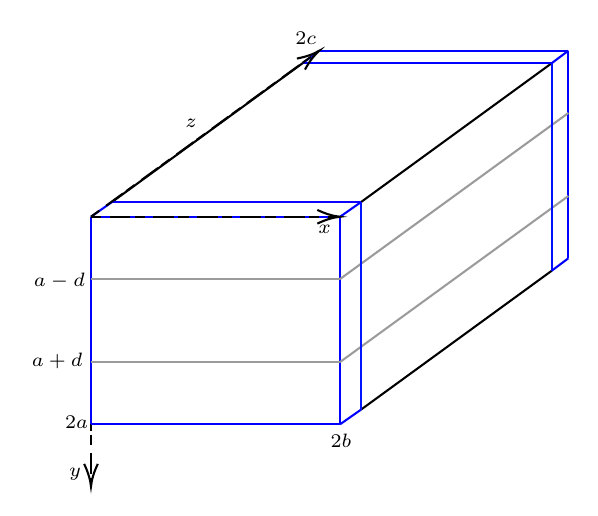
\begin{tikzpicture}[x=0.75pt,y=0.75pt,yscale=-1,xscale=1]
%uncomment if require: \path (0,461); %set diagram left start at 0, and has height of 461

%Straight Lines [id:da33793160626814234] 
\draw [color={rgb, 255:red, 0; green, 0; blue, 0 }  ,draw opacity=1 ] [dash pattern={on 3.75pt off 3pt on 7.5pt off 1.5pt}]  (60,120) -- (60,248) ;
\draw [shift={(60,250)}, rotate = 270] [color={rgb, 255:red, 0; green, 0; blue, 0 }  ,draw opacity=1 ][line width=0.75]    (10.93,-3.29) .. controls (6.95,-1.4) and (3.31,-0.3) .. (0,0) .. controls (3.31,0.3) and (6.95,1.4) .. (10.93,3.29)   ;
%Straight Lines [id:da21048665747646944] 
\draw    (70,113) -- (162,46) ;
%Straight Lines [id:da21496427185008327] 
\draw    (190,113) -- (282,46) ;
%Straight Lines [id:da04028217537075074] 
\draw [color={rgb, 255:red, 0; green, 0; blue, 255 }  ,draw opacity=1 ]   (60,120) -- (180,120) ;
%Straight Lines [id:da7170712168727287] 
\draw [color={rgb, 255:red, 0; green, 0; blue, 255 }  ,draw opacity=1 ]   (170,40) -- (290,40) ;
%Straight Lines [id:da12233767000161122] 
\draw [color={rgb, 255:red, 0; green, 0; blue, 255 }  ,draw opacity=1 ]   (60,220) -- (180,220) ;
%Straight Lines [id:da3869762813522424] 
\draw    (190,213) -- (282,146) ;
%Straight Lines [id:da05729970060070899] 
\draw [color={rgb, 255:red, 0; green, 0; blue, 255 }  ,draw opacity=1 ]   (60,120) -- (60,220) ;
%Straight Lines [id:da881902696420134] 
\draw [color={rgb, 255:red, 0; green, 0; blue, 255 }  ,draw opacity=1 ]   (180,120) -- (180,220) ;
%Straight Lines [id:da30748964416540847] 
\draw [color={rgb, 255:red, 0; green, 0; blue, 255 }  ,draw opacity=1 ]   (290,40) -- (290,140) ;
%Straight Lines [id:da4970694191237319] 
\draw [color={rgb, 255:red, 155; green, 155; blue, 155 }  ,draw opacity=1 ]   (60,150) -- (180,150) ;
%Straight Lines [id:da2761427702849881] 
\draw [color={rgb, 255:red, 155; green, 155; blue, 155 }  ,draw opacity=1 ]   (60,190) -- (180,190) ;
%Straight Lines [id:da8026720700371979] 
\draw [color={rgb, 255:red, 155; green, 155; blue, 155 }  ,draw opacity=1 ]   (180,190) -- (290,110) ;
%Straight Lines [id:da23722210789790243] 
\draw [color={rgb, 255:red, 155; green, 155; blue, 155 }  ,draw opacity=1 ]   (180,150) -- (290,70) ;
%Straight Lines [id:da9998354929478732] 
\draw [color={rgb, 255:red, 13; green, 0; blue, 255 }  ,draw opacity=1 ]   (70,113) -- (190,113) ;
%Straight Lines [id:da4132700627297399] 
\draw [color={rgb, 255:red, 0; green, 0; blue, 255 }  ,draw opacity=1 ]   (162,46) -- (282,46) ;
%Straight Lines [id:da5939794577660118] 
\draw [color={rgb, 255:red, 0; green, 20; blue, 255 }  ,draw opacity=1 ]   (190,113) -- (190,213) ;
%Straight Lines [id:da8623036562152813] 
\draw [color={rgb, 255:red, 0; green, 15; blue, 255 }  ,draw opacity=1 ]   (282,46) -- (282,146) ;
%Straight Lines [id:da8793888735498807] 
\draw [color={rgb, 255:red, 0; green, 0; blue, 255 }  ,draw opacity=1 ]   (180,120) -- (190,113) ;
%Straight Lines [id:da6169914746452605] 
\draw [color={rgb, 255:red, 0; green, 0; blue, 255 }  ,draw opacity=1 ]   (180,220) -- (190,213) ;
%Straight Lines [id:da8616702568255465] 
\draw [color={rgb, 255:red, 0; green, 0; blue, 255 }  ,draw opacity=1 ]   (60,120) -- (70,113) ;
%Straight Lines [id:da7336605374589271] 
\draw [color={rgb, 255:red, 0; green, 0; blue, 255 }  ,draw opacity=1 ]   (282,146) -- (290,140) ;
%Straight Lines [id:da4871143624254335] 
\draw [color={rgb, 255:red, 0; green, 0; blue, 255 }  ,draw opacity=1 ]   (282,46) -- (290,40) ;
%Straight Lines [id:da6094463937535262] 
\draw [color={rgb, 255:red, 0; green, 0; blue, 255 }  ,draw opacity=1 ]   (162,46) -- (170,40) ;
%Straight Lines [id:da8435206245989231] 
\draw [color={rgb, 255:red, 0; green, 0; blue, 0 }  ,draw opacity=1 ] [dash pattern={on 3.75pt off 3pt on 7.5pt off 1.5pt}]  (60,120) -- (178,120) ;
\draw [shift={(180,120)}, rotate = 180] [color={rgb, 255:red, 0; green, 0; blue, 0 }  ,draw opacity=1 ][line width=0.75]    (10.93,-3.29) .. controls (6.95,-1.4) and (3.31,-0.3) .. (0,0) .. controls (3.31,0.3) and (6.95,1.4) .. (10.93,3.29)   ;
%Straight Lines [id:da416605107929652] 
\draw [color={rgb, 255:red, 0; green, 0; blue, 0 }  ,draw opacity=1 ] [dash pattern={on 3.75pt off 3pt on 7.5pt off 1.5pt}]  (60,120) -- (168.38,41.18) ;
\draw [shift={(170,40)}, rotate = 143.97] [color={rgb, 255:red, 0; green, 0; blue, 0 }  ,draw opacity=1 ][line width=0.75]    (10.93,-3.29) .. controls (6.95,-1.4) and (3.31,-0.3) .. (0,0) .. controls (3.31,0.3) and (6.95,1.4) .. (10.93,3.29)   ;

% Text Node
\draw (168,122.4) node [anchor=north west][inner sep=0.75pt]  [font=\scriptsize]  {$x$};
% Text Node
\draw (48,239.4) node [anchor=north west][inner sep=0.75pt]  [font=\scriptsize]  {$y$};
% Text Node
\draw (104,71.4) node [anchor=north west][inner sep=0.75pt]  [font=\scriptsize]  {$z$};
% Text Node
\draw (46,214.4) node [anchor=north west][inner sep=0.75pt]  [font=\scriptsize]  {$2a$};
% Text Node
\draw (31,145.4) node [anchor=north west][inner sep=0.75pt]  [font=\scriptsize]  {$a-d$};
% Text Node
\draw (30,184.4) node [anchor=north west][inner sep=0.75pt]  [font=\scriptsize]  {$a+d$};
% Text Node
\draw (174,223.4) node [anchor=north west][inner sep=0.75pt]  [font=\scriptsize]  {$2b$};
% Text Node
\draw (157,29.4) node [anchor=north west][inner sep=0.75pt]  [font=\scriptsize]  {$2c$};


\end{tikzpicture}

Slicing a plane $xy$ on half-length of $z$-axis:



\tikzset{every picture/.style={line width=0.75pt}} %set default line width to 0.75pt        

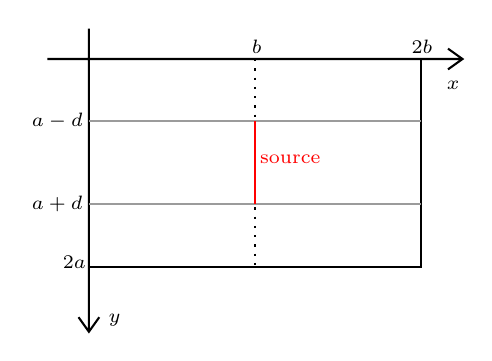
\begin{tikzpicture}[x=0.75pt,y=0.75pt,yscale=-1,xscale=1]
%uncomment if require: \path (0,300); %set diagram left start at 0, and has height of 300

%Straight Lines [id:da3480880018545507] 
\draw  [dash pattern={on 0.84pt off 2.51pt}]  (120,30) -- (120,130) ;
%Shape: Axis 2D [id:dp3637924149326488] 
\draw  (40,15.4) -- (40,161.4)(220,30) -- (20,30) (45,154.4) -- (40,161.4) -- (35,154.4) (213,25) -- (220,30) -- (213,35)  ;
%Shape: Rectangle [id:dp609433285561545] 
\draw   (40,30) -- (200,30) -- (200,130) -- (40,130) -- cycle ;
%Straight Lines [id:da15540762860028612] 
\draw [color={rgb, 255:red, 155; green, 155; blue, 155 }  ,draw opacity=1 ]   (40,60) -- (200,60) ;
%Straight Lines [id:da5236995862324196] 
\draw [color={rgb, 255:red, 155; green, 155; blue, 155 }  ,draw opacity=1 ]   (40,100) -- (200,100) ;
%Straight Lines [id:da00556491703537243] 
\draw [color={rgb, 255:red, 255; green, 0; blue, 0 }  ,draw opacity=1 ]   (120,60) -- (120,100) ;

% Text Node
\draw (211,39.4) node [anchor=north west][inner sep=0.75pt]  [font=\scriptsize]  {$x$};
% Text Node
\draw (48,151.4) node [anchor=north west][inner sep=0.75pt]  [font=\scriptsize]  {$y$};
% Text Node
\draw (194,19.4) node [anchor=north west][inner sep=0.75pt]  [font=\scriptsize]  {$2b$};
% Text Node
\draw (26,123.4) node [anchor=north west][inner sep=0.75pt]  [font=\scriptsize]  {$2a$};
% Text Node
\draw (117,19.4) node [anchor=north west][inner sep=0.75pt]  [font=\scriptsize]  {$b$};
% Text Node
\draw (11,54.4) node [anchor=north west][inner sep=0.75pt]  [font=\scriptsize]  {$a-d$};
% Text Node
\draw (11,94.4) node [anchor=north west][inner sep=0.75pt]  [font=\scriptsize]  {$a+d$};
% Text Node
\draw (121,75) node [anchor=north west][inner sep=0.75pt]  [font=\scriptsize,color={rgb, 255:red, 255; green, 0; blue, 0 }  ,opacity=1 ] [align=left] {source};


\end{tikzpicture}

Slicing a plane $zy$ on half-length of $x$-axis:



% Pattern Info
 
\tikzset{
pattern size/.store in=\mcSize, 
pattern size = 5pt,
pattern thickness/.store in=\mcThickness, 
pattern thickness = 0.3pt,
pattern radius/.store in=\mcRadius, 
pattern radius = 1pt}
\makeatletter
\pgfutil@ifundefined{pgf@pattern@name@_64w1ndx3q}{
\pgfdeclarepatternformonly[\mcThickness,\mcSize]{_64w1ndx3q}
{\pgfqpoint{0pt}{-\mcThickness}}
{\pgfpoint{\mcSize}{\mcSize}}
{\pgfpoint{\mcSize}{\mcSize}}
{
\pgfsetcolor{\tikz@pattern@color}
\pgfsetlinewidth{\mcThickness}
\pgfpathmoveto{\pgfqpoint{0pt}{\mcSize}}
\pgfpathlineto{\pgfpoint{\mcSize+\mcThickness}{-\mcThickness}}
\pgfusepath{stroke}
}}
\makeatother

% Pattern Info
 
\tikzset{
pattern size/.store in=\mcSize, 
pattern size = 5pt,
pattern thickness/.store in=\mcThickness, 
pattern thickness = 0.3pt,
pattern radius/.store in=\mcRadius, 
pattern radius = 1pt}
\makeatletter
\pgfutil@ifundefined{pgf@pattern@name@_qnc3ayslt}{
\pgfdeclarepatternformonly[\mcThickness,\mcSize]{_qnc3ayslt}
{\pgfqpoint{0pt}{-\mcThickness}}
{\pgfpoint{\mcSize}{\mcSize}}
{\pgfpoint{\mcSize}{\mcSize}}
{
\pgfsetcolor{\tikz@pattern@color}
\pgfsetlinewidth{\mcThickness}
\pgfpathmoveto{\pgfqpoint{0pt}{\mcSize}}
\pgfpathlineto{\pgfpoint{\mcSize+\mcThickness}{-\mcThickness}}
\pgfusepath{stroke}
}}
\makeatother
\tikzset{every picture/.style={line width=0.75pt}} %set default line width to 0.75pt        

\begin{tikzpicture}[x=0.75pt,y=0.75pt,yscale=-1,xscale=1]
%uncomment if require: \path (0,300); %set diagram left start at 0, and has height of 300

%Shape: Rectangle [id:dp6810885499420589] 
\draw  [color={rgb, 255:red, 0; green, 0; blue, 255 }  ,draw opacity=1 ][pattern=_64w1ndx3q,pattern size=6pt,pattern thickness=0.75pt,pattern radius=0pt, pattern color={rgb, 255:red, 0; green, 0; blue, 255}] (180,30) -- (200,30) -- (200,130) -- (180,130) -- cycle ;
%Shape: Rectangle [id:dp9654892852591364] 
\draw  [color={rgb, 255:red, 0; green, 0; blue, 255 }  ,draw opacity=1 ][pattern=_qnc3ayslt,pattern size=6pt,pattern thickness=0.75pt,pattern radius=0pt, pattern color={rgb, 255:red, 0; green, 0; blue, 255}] (40,30) -- (60,30) -- (60,130) -- (40,130) -- cycle ;
%Straight Lines [id:da3480880018545507] 
\draw  [dash pattern={on 0.84pt off 2.51pt}]  (120,30) -- (120,130) ;
%Shape: Axis 2D [id:dp3637924149326488] 
\draw  (40,15.4) -- (40,161.4)(220,30) -- (20,30) (45,154.4) -- (40,161.4) -- (35,154.4) (213,25) -- (220,30) -- (213,35)  ;
%Shape: Rectangle [id:dp609433285561545] 
\draw   (40,30) -- (200,30) -- (200,130) -- (40,130) -- cycle ;
%Straight Lines [id:da15540762860028612] 
\draw [color={rgb, 255:red, 155; green, 155; blue, 155 }  ,draw opacity=1 ]   (40,60) -- (200,60) ;
%Straight Lines [id:da5236995862324196] 
\draw [color={rgb, 255:red, 155; green, 155; blue, 155 }  ,draw opacity=1 ]   (40,100) -- (200,100) ;
%Straight Lines [id:da00556491703537243] 
\draw [color={rgb, 255:red, 255; green, 0; blue, 0 }  ,draw opacity=1 ]   (120,60) -- (120,100) ;

% Text Node
\draw (211,39.4) node [anchor=north west][inner sep=0.75pt]  [font=\scriptsize]  {$z$};
% Text Node
\draw (48,151.4) node [anchor=north west][inner sep=0.75pt]  [font=\scriptsize]  {$y$};
% Text Node
\draw (194,19.4) node [anchor=north west][inner sep=0.75pt]  [font=\scriptsize]  {$2c$};
% Text Node
\draw (26,123.4) node [anchor=north west][inner sep=0.75pt]  [font=\scriptsize]  {$2a$};
% Text Node
\draw (117,19.4) node [anchor=north west][inner sep=0.75pt]  [font=\scriptsize]  {$c$};
% Text Node
\draw (11,54.4) node [anchor=north west][inner sep=0.75pt]  [font=\scriptsize]  {$a-d$};
% Text Node
\draw (11,94.4) node [anchor=north west][inner sep=0.75pt]  [font=\scriptsize]  {$a+d$};
% Text Node
\draw (121,75) node [anchor=north west][inner sep=0.75pt]  [font=\scriptsize,color={rgb, 255:red, 255; green, 0; blue, 0 }  ,opacity=1 ] [align=left] {source};
% Text Node
\draw (202,75) node [anchor=north west][inner sep=0.75pt]  [font=\scriptsize,color={rgb, 255:red, 0; green, 0; blue, 255 }  ,opacity=1 ] [align=left] {PML};
% Text Node
\draw (62,75) node [anchor=north west][inner sep=0.75pt]  [font=\scriptsize,color={rgb, 255:red, 0; green, 0; blue, 255 }  ,opacity=1 ] [align=left] {PML};


\end{tikzpicture}

Consider the parameters:

\begin{table}[H]
    \centering
    \begin{tabular}{|c|c|c|}
    \hline
    \textbf{Parameter} & \textbf{Description}               & \textbf{Value} \\ \hline
    $a$                & Half-length on $y$-axis              & 5 cm           \\ \hline
    $b$                & Half-length on $x$-axis              & 5 cm           \\ \hline
    $c$                & Half-length on $z$-axis              & 10 cm          \\ \hline
    $d$                & Half-distance between strips       & 2 cm           \\ \hline
    $N_x$              & Number of cells on $x$-axis          & 40             \\ \hline
    $N_y$              & Number of cells on $y$-axis          & 40             \\ \hline
    $N_z$              & Number of cells on $z$-axis          & 70             \\ \hline
    $N_{\textnormal{PML}}$          & Number of cells with PML on z-axis & 10             \\ \hline
    $\epsilon_{r_2}$          & Relative permittivity between strips & 5             \\ \hline
    \end{tabular}
\end{table}

From this table it is possible to derive other parameters:

\begin{table}[H]
    \centering
    \begin{tabular}{|c|c|c|}
    \hline
    \textbf{Parameter}                           & \textbf{Description} & \textbf{Value} \\ \hline
    $N_x^c$                                      & Index centered on x  & 20             \\ \hline
    $N_y^c$                                      & Index centered on y  & 20             \\ \hline
    $N_z^c$                                      & Index centered on z  & 35             \\ \hline
    $N_{\textnormal{plate}}^{\textnormal{high}}$ & Y-index of top strip & 32             \\ \hline
    $N_{\textnormal{plate}}^{\textnormal{low}}$  & Y-index of low strip & 8              \\ \hline
    $\dx$                                        & ${2b}/{N_x}$         & 40             \\ \hline
    $\dy$                                        & ${2a}/{N_y}$         & 70             \\ \hline
    $\dz$                                        & ${2c}/{N_z}$         & 10             \\ \hline
    \end{tabular}
\end{table}

\subsection{Boundary Conditions}

\subsubsection{On Source} \hfill

The source is located at $\pare{N_x^c, N_{\textnormal{plate}}^{\textnormal{low}} : N_{\textnormal{plate}}^{\textnormal{high}}, N_z^c}$. It will be considered that the source is on $\En_y$ as shown below: 

\begin{figure}[H]
    \centering
    \includegraphics[width=0.45\textwidth]{contents/input_source.png}
    \caption{Input electric field with frequency $f_c = \SI{3.0}{\giga\hertz}$, peak time $t_p = \SI{1.5}{\nano\second}$ and duration $t_f = \SI{5.0}{\nano\second}$. The Gaussian that limits the sine function has $\tau = \SI{0.5}{\nano\second}$.}
\end{figure}

\subsubsection{On Conductor Strips}\hfill

There is one strip located at $\pare{:, N_{\textnormal{plate}}^{\textnormal{low}}, :}$ and another at $\pare{:, N_{\textnormal{plate}}^{\textnormal{high}}, :}$. At these positions is valid:

\begin{align}
    \En_x = \En_z = \Hht_y = 0
\end{align}

\subsubsection{Conductor Walls}\hfill

The condition for conductor walls is the same as for conductor strips. Their positions are at: $\pare{0, :, :}$, $\pare{N_x-1, :, :}$, $\pare{:, 0, :}$,$\pare{:, N_y-1, :}$, $\pare{:, :, 0}$ and $\pare{:, :, N_z-1}$.

\subsection{Step Time}

The step time was chosen to obey the Courant Stability condition:

\begin{equation}
    \dt \leq \cfrac{1}{c_0\sqrt{\pare{\cfrac{1}{\dx}}^2 + \pare{\cfrac{1}{\dy}}^2 + \pare{\cfrac{1}{\dz}}^2}}
\end{equation}

\subsection{Simulation Results}

\begin{figure}[H]
    \centering
    \includegraphics[width=0.45\textwidth]{contents/central_xy_plane.png}
    \caption{Central XY Plane.}
\end{figure}

\begin{figure}[H]
    \centering
    \includegraphics[width=0.45\textwidth]{contents/central_zy_plane.png}
    \caption{Central ZY Plane.}
\end{figure}